\documentclass{article}
\usepackage[utf8]{inputenc}
\usepackage[dvipdfmx]{hyperref}
\usepackage{fancyhdr}
\usepackage{caption, floatrow}

\usepackage[dvipdfmx]{graphicx}

\usepackage{mathtools}
\renewcommand{\theequation}{eq. \arabic{equation}}


\usepackage[
  style=numeric,
  citestyle=numeric,
  url=true,
  doi=false,
  isbn=false
  ]{biblatex}
\addbibresource{main.bib}


\DeclareNewFloatType{graph}{placement=H, name=Graph}
\floatsetup[graph]{capposition=bottom}


% contents below
% ------------------------------------------------------------------------------

\pagestyle{fancy}
\fancyhf{}
\rhead{Rikuo Hasegawa}
\chead{UPCSE PHYSICS Short Lab Report}
\lhead{\today}
\rfoot{p. \thepage}

\title{Photoelectric Effect}
\author{ Rikuo Hasegawa
  \\ Tutorial Group: C
  \\ Lab Group: C2 }

\begin{document}

\maketitle
\thispagestyle{fancy}
\vspace*{\fill}
\parbox{\linewidth}{\centering%
Date of Experiment: February 6th, 2019
}
\newpage


\section{Introduction}

In this experiment our goal is to measure the planck constant by examining the photoelectric effect using a halogen lamp and a PASCO h/e apparatus. We also want to measure the work function of the metal in the PASCO apparatus.

\section{Theory}

The energy of a photon is given in \eqref{eq:photon}

\begin{equation}\label{eq:photon}
  E = hf
\end{equation}

When photons with enough energy collide with a metal surface, it can cause electrons to be emitted. These electrons are sometimes referred to as photoelectrons. Each metal has a property which describes the amount of energy required before an electron gets emitted. This value is called the Work Function of the metal and is expressed using the symbol $\Phi$. The kinetic energy of a photoelectron is given in \eqref{eq:photo_ke}

\begin{equation}\label{eq:photo_ke}
  KE_{max} = hf - \Phi
\end{equation}

By measuring the voltage $V_s$ of the emitted electrons, we can also find the kinetic energy as given in \eqref{eq:volt_ke}.

\begin{equation}\label{eq:volt_ke}
  KE_{max} = e V_s
\end{equation}
where $e$ is the charge of an electron, which is $1.60217662 \times 10^{-19}$ \autocite{mohr_2016}.

\section{Experimental Equipment and Method}
\subsection{Apparatus}

Shown below is our experiment apparatus in Figure \ref{fig:apparatus}.

\begin{figure}
  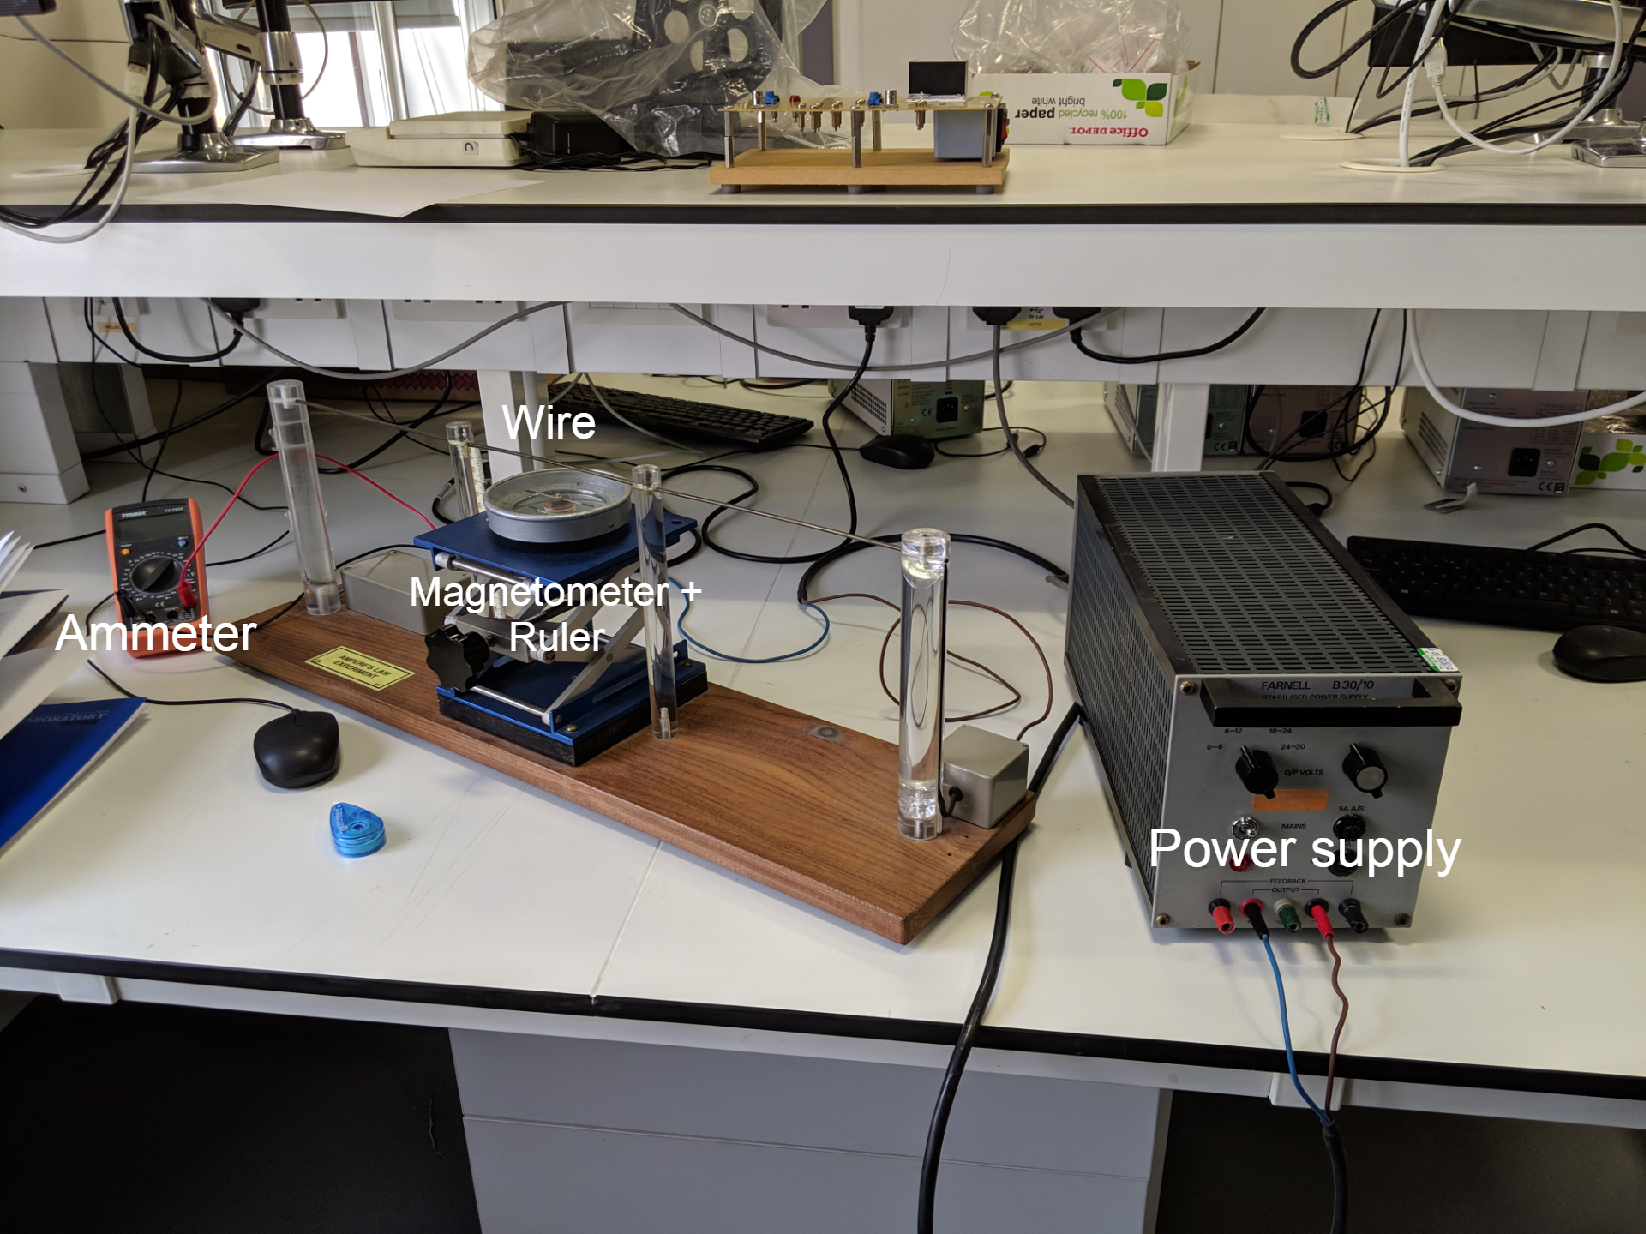
\includegraphics{./img/apparatus.pdf}
  \caption{\autocite{UPCSE2018}}
  \label{fig:apparatus}
\end{figure}

\paragraph{}
The equipment we used consists of several main components:
\begin{enumerate}
  \item Halogen lamp as a source of white light
  \item Convex lens to focus light onto PASCO apparatus
  \item Filters of specific wavelength to limit frequency of light entering apparatus
  \item PASCO h/e measurement apparatus
  \item Digital Voltmeter to read values from PASCO apparatus
\end{enumerate}
The uncertainty on the voltmeter is $1 \times 10^{-3}$ [V]. We used filters of wavelength 400, 410, 440, 520, 546, and 600 [nm]. The uncertainty on these are $5 \times 10^{-10}$ [m].

\subsection{Protocol}

The experiment protocol is described below:

\begin{enumerate}
  \item Turn on the halogen lamp and focus the light onto the PASCO device using the convex lens.
  \item Turn on the PASCO device and the voltmeter.
  \item Main loop, begin with 400 nm filter and move up:
  \begin{enumerate}
    \item Insert the filter into the filter holder.
    \item Press the PRESS TO ZERO button on the PASCO device.
    \item Take measurement on voltmeter.
  \end{enumerate}
  \item Repeat main loop using other filter wavelengths.
  \item Turn all devices off.
\end{enumerate}

\section{Results}
\paragraph{}
Our raw data is shown in Table \ref{tb:data}.
\begin{table}[h]
  \includegraphics{./img/table_data.pdf}
  \caption{Raw measurements}
  \label{tb:data}
\end{table}
By plotting the $eV_s$ against the frequency of light, we will be graphing \eqref{eq:final}, which can be derived from \eqref{eq:photo_ke} and \eqref{eq:volt_ke}.

\begin{equation}\label{eq:final}
  eV_s = hf - \Phi
\end{equation}

\begin{graph}[H]
  \includegraphics{./img/graph.pdf}
  \caption{$eV_s$ against frequency}
  \label{fig:graph}
\end{graph}

The gradient of this graph should provide us with the Planck Constant and the y-intercept should provide us with the work function $\Phi$ of the metal in the PASCO device.

\section{Uncertainty Analysis}

Using the regression feature of the data analysis toolkit in Microsoft Excel, we calculated the uncertainty in our measurements.

\begin{table}[h]
  \includegraphics{./img/table_uncertainty.pdf}
  \caption{Uncertainty analysis}
  \label{tb:uncertainty}
\end{table}

Thus, our measurements for the Planck Constant $h$ and the work function $\Phi$ are as follows:

$$
h = 5.63 \pm 2.49 \times 10^{-34} \text{[m$^2$ kg/s]}
$$
$$
\Phi = -1.10 \pm 1.58 \times 10^{-19} \text{[J]}
$$

The known value of the Planck Constant is $h = 6.6260693 \times 10^{-34}$ \autocite{mohr_2016}. Our measurements do contain this value, so we have successfully measured the planck constant. However, with regard to both measurements, especially the work function, our random errors are very high.

\section{Discussion and Conclusion}
\paragraph{}
One of the most probable causes of the large uncertainty is that there were gaps in the filter for some of the filters, which would enable light of other frequencies to enter the PASCO device. This would render the measurements useless for the filters with this particular defect.

This experiment was successful in measuring the Planck Constant, albeit with a worryingly large uncertainty. With the work function of the metal, it is difficult to say that our experiment measured the value, as the work function cannot be negative.

\section{Appendix}

It is initially unintuitive that only frequency affects the voltage of photoelectrons. In order to rule out the effect of intensity of light, we took measurements with a filter which reduces the intesity of light regardless of wavelength. The observed voltage was not affected, as would be expected by the theory.

\printbibliography
\end{document}
